% !TEX encoding = UTF-8
% !TEX program = pdflatex
% !TEX root = MEMOC.tex
% !TEX spellcheck = it-IT

% 11 Novembre 2016
%\chapter{Meta-euristiche}
%\section{Local Search}
%\subsection{Esempio di Local Search su TSP}

\section{Neighbourhood search e Trajectory methods}

La ricerca locale costituisce un buon trade-off tra la semplicità e l'efficienza, ma c'è il rischio che si blocchi su un ottimo locale.
Serve quindi una strategia per \textit{schivare} questi ottimi. Da notare che se la funzione da ottimizzare è convessa, non c'è questo problema perché ogni ottimo locale è anche globale. Tipicamente questo non si verifica nei problemi di ottimizzazione.

Alcune idee possono essere quelle di fare i riavvi casuali, cambiare la dimensione del vicinato, randomizzare l'esplorazione o effettuare backtrack. Ma questi modi permettono solamente di ripartire una volta incastrati.

Un'approccio alternativo è quello dei \textbf{trajectory methods}, i quali continuano l'esplorazione dello spazio delle soluzioni anche dopo essere finiti in un ottimo locale.
Per fare ciò è necessario ammettere delle mosse che portano ad una soluzione peggiore.

Con questa strategia c'è il rischio di finire in un loop. Per evitare ciò è possibile:

\begin{itemize}
	\item Accettare solamente soluzioni migliori. Ad esempio: \textit{Hill Climbing}
	\item Esplorare in modo randomizzato lo spazio, senza sfruttare le informazioni sul problema. Ad esempio: \textit{Simulated Annealing}.
	\item Tenere traccia delle soluzioni che sono già state incontrate, sfruttando la struttura del problema. Ad esempio: \textit{Tabu Search}
\end{itemize}

\noindent Da notare che finire più volte sulla stessa soluzione può essere accettabile. In questo caso è però necessario evitare di scegliere ancora lo stesso vicino precedentemente scelto.

\subsection{Simulated Annealing}

Questo metodo deriva dal processo di annealing del vetro e metallo.

\begin{enumerate}
	\item Determina una soluzione iniziale $x$. $x* \leftarrow x$, $k=0$.
	\item Ripeti finché non ci sono più vicino o hai fatto un certo numero di iterazioni:
		\begin{itemize}
			\item $k \leftarrow k +1$.
			\item Genera un vicino casuale $y$.
			\item Se il vicino $y$ è migliore di $x*$, $x* \leftarrow y$.
			\item Altrimenti calcola
			$$
			p = \min \bigg\{1, exp\bigg(-\frac{f(y)-f(x)}{T(k)}\bigg)\bigg\}
			$$
			e accetta $y$ con probabilità $p$.
			\item Se hai accettato $y$, $x* \leftarrow y$.
		\end{itemize}
	\item Ritorna $x*$.
\end{enumerate}

\noindent Il parametro $T(k)$ rappresenta la temperatura del processo, più alto è e più è probabile accettare soluzioni peggiori. Man mano che l'esecuzione avanza la temperatura cala.

A livello teorico è possibile provare che sotto alcune assunzioni (un tempo di raffreddamento molto lungo) questo metodo riesce a convergere ad un ottimo globale.
Ma a livello pratico ci sono delle meta-euristiche che funzionano meglio.

\subsection{Tabu Search}

Questa ricerca utilizza la memorizzazione delle soluzioni per evitare di ciclare.
L'idea di base è quella di escludere (fare Tabu) le soluzioni già visitate dai vicinati.

Durante l'esecuzione viene manutenuta una \textbf{Tabu List}, una lista che contiene le ultime \textit{t} soluzioni visitate.

$$
T(k) := \{x^{k-1}, x^{k-2}, \ldots, x^{k-t} \}
$$

\noindent Così facendo all'iterazione $k$ vengono evitati cicli di lunghezza $\leq t$, dove $t$ è un parametro che deve essere calibrato.
La limitazione data dal parametro $t$ è presente per limitare il consumo di memoria e per rendere la ricerca sulla lista più veloce.

La generazione del vicinato adesso viene effettuata da una funzione $N(x,k)$ che tiene anche conto dell'iterazione per evitare i tabu.

Per aumentare l'efficienza ed occupare meno spazio si può scegliere di tenere traccia delle mosse effettuate (o di qualche altra caratteristica) al posto della soluzione, perché può essere che valutare l'uguaglianza di due soluzioni sia troppo costoso o perché una singola soluzione richiede troppa memoria.
C'è però uno svantaggio nel tenere traccia delle mosse, perché potrebbero venire escluse delle soluzioni che non sono ancora state visitate.

Si possono quindi definire degli \textbf{aspiration criteria} che se vengono soddisfatti sorpassano la regola del tabu e lasciano visitare comunque la soluzione. Ad esempio come aspiration criteria si può utilizzare ``\textit{la soluzione tabu ha il valore migliore di funzione obiettivo tra tutti quelle visitate finora}''.

La ricerca Tabu può essere fermata quando:

\begin{itemize}
	\item Viene trovata una soluzione che può essere provata ottima (in qualche modo).
	\item Viene raggiunto un numero massimo di iterazioni o un tempo massimo.
	\item Dopo aver trovato un certo numero di soluzioni che non hanno migliorato la funzione obiettivo.
	\item Non ci sono più vicini e non è possibile applicare un aspiration criteria. Può essere dovuto ad un $t$ troppo alto.
\end{itemize}

\noindent Lo schema dell'algoritmo è il seguente:

\begin{enumerate}
	\item Determina una soluzione di partenza $x$. $k \leftarrow 0$, $T(k) = \emptyset$, $x* \leftarrow x$.
	\item Ripeti finché non vale il criterio di arresto scelto:
	\begin{itemize}
		\item $$
		y = \arg \text{best} \bigg( \Big\{ \overline{f}(y), y \in N(x,k) \Big\} \cup \Big\{ y \in N(x) \setminus N(x,k) : y \text{ soddisfa un criterio di aspirazione}\Big\} \bigg)
		$$
		\item Calcola $T(k+1)$ aggiungendo $y$ alla lista. Se necessario rimuovi dalla lista la soluzione più vecchia.
		\item Se $f(y)$ migliora $f(x*)$, $x* \leftarrow y$.
		\item $x \leftarrow y$, $k\text{++}$.
	\end{itemize}
	\item Ritorna $x*$.
\end{enumerate}

\section{Intesification e Diversification Phase}

Ci passiamo sopra veloce, leggi dalle slide

\section{Euristiche basate sulla popolazione - Algoritmi genetici}

Nella ricerca sul vicinato viene esplorato lo spazio delle soluzioni secondo un certo percorso.

Nei metodi basati sulla popolazione, ad ogni iterazione viene preso in considerazione un set di soluzioni, che prende il nome di \textbf{popolazione}. Per ottenere delle nuove soluzioni, vengono prese due soluzioni dalla popolazione e vengono combinate tra loro per ottenere un soluzione (sperabilmente migliore).

La metafora di questa meta-euristica deriva dalla teoria Darwiniana, dove la sopravvivenza del \textit{fittest} diventa il processo di ottimizzazione dell'individuo. L'individuo è la soluzione e il livello di \textit{fitness} è dato dalla funzione obiettivo.

Lo schema di questa famiglia di algoritmi è il seguente:

\begin{enumerate}
	\item Codifica le soluzioni per il problema specifico.
	\item Crea un set iniziale di soluzioni (\textbf{initail population}).
	\item Ripeti finché non viene raggiunto un criterio di stop:
	\begin{itemize}
		\item Selezione delle coppie o gruppi di soluzioni (\textbf{parents}).
		\item Ricombina i \textbf{partens} per generare delle nuove soluzioni \textbf{offspring}.
		\item Valuta il fitness delle nuove soluzioni.
		\item Rimpiazza la popolazione, utilizzando la nuova generazione. 
	\end{itemize}
	\item Ritorna la soluzione migliore che è stata generata.
\end{enumerate}

\noindent Il tutto funziona perché tipicamente combinando due elementi forti, si ottiene un figlio che è ancora più forte, il quale va ad alzare il livello medio della popolazione.

\subsection{Codifica della soluzione}

L'encoding della soluzione varia da problema a problema, ad esempio per KP0/1 possiamo usare un vettore binario o per TSP possiamo usare un vettore con l'ordine di visita dei nodi. Ogni caratteristica della codifica prende il nome di \textbf{gene}.

\subsection{Operazioni genetiche}

\subsubsection{Creazione della popolazione iniziale}

Il set di iniziale è importante che sia il più vario possibile e può essere generato utilizzando altre meta-euristiche randomizzate. \`E molto importante il focus sulla diversificazione.

\subsubsection{Fitness}

Può essere la funzione obiettivo o una sua variante con delle penalizzazioni.

\subsubsection{Selezione}

La selezione dovrebbe dare una probabilità maggiore alle soluzioni migliori, ma anche quelle peggiori devono avere la possibilità di essere scelte, in modo da evitare una convergenza troppo veloce.
Alcuni metodi sono: Montecarlo, Linear Ranking, n-tournament.

\subsubsection{Riproduzione}

Da $n$ genitori è possibile ottenere $m$ figli diversi ma simili.

Un modo può generare i figli è di scegliere i geni dai vari genitori, dando maggiore probabilità di scelta ai geni dei genitori migliori (\textbf{uniform}).
Un'alternativa è quella di ereditare i geni dai genitori ``\textit{a blocchi}'' (\textbf{k-cut-point}).

\begin{figure}[htbp]
	\centering
	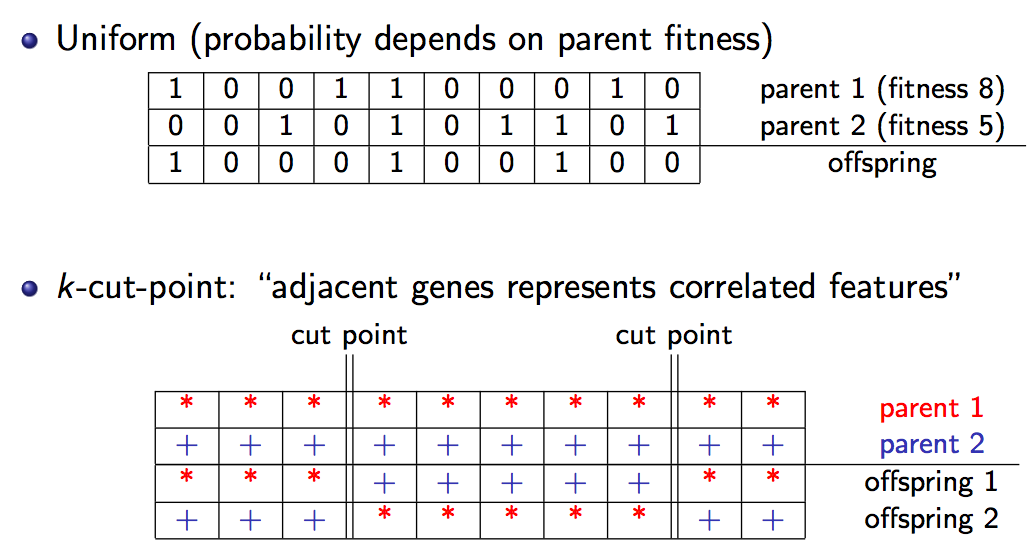
\includegraphics[width=0.7\textwidth]{images/l8-fig-1.png}
\end{figure}

\subsubsection{Mutazione}

Una chiave del processo evolutivo sono le mutazioni casuali, le quali devono essere codificate anche all'interno dell'algoritmo durante il processo di riproduzione o subito dopo.

La mutazione viene replicata andando a modificare casualmente alcuni geni della nuova generazione.
Questo evita che si crei un \textbf{genetic drift}, ovvero una popolazione in cui tutti gli individui hanno lo stesso valore per alcuni geni.

Così facendo viene reintrodotta la diversificazione dei geni e rallentata la convergenza della popolazioni. Si può poi utilizzare una mutazione più spinta per diversificare ancora di più la popolazione.

\subsubsection{Local Search per l'educazione dei figli}

Volendo si può utilizzare la ricerca locale per migliorare la nuova generazione, rimpiazzando il nuovo individuo con il suo minimo locale.

Bisogna però stare attenti all'efficienza, perché la ricerca locale potrebbe richiedere troppo tempo. Volendo si può fare solo ad un sotto-insieme della nuova generazione.

\subsubsection{Riproduzione e mutazioni che generano figli malformati}

Sia la riproduzione che le mutazioni possono creare un figlio che è infeasible (non è una soluzione valida).

Si può quindi scegliere di scartare il figlio (THIS IS SPARTA!), penalizzargli la funzione di fitness oppure di ripararlo e trasformarlo in una soluzione feasible.

Un'altra idea è quella di prevenire questi casi, definendo delle operazioni specifiche che mantengono la feasibility della soluzione.

\subsection{Osservazioni}

Questi algoritmi sono molto generici, robusti e adattabili su molti contesti, infatti molti risolutori permetto di utilizzarli.

C'è però lo svantaggio che vengono richiesti molti parametri che devono essere calibrati dall'utilizzatore dell'algoritmo. Quindi il problema non è più ``trovare una soluzione'' ma è quello di trovare i parametri ottimi.

Gli algoritmi genetici vengono detti \textbf{weak methods} o \textbf{soft computing} perché non richiedono conoscenze specifiche riguardo il problema.

\`E importante che l'ideatore dell'algoritmo fornisca anche i parametri ottimi.






